%% Package and Class "uiucthesis2014" for use with LaTeX2e.
\documentclass[edeposit,fullpage]{uiucthesis2018}


\usepackage[acronym,toc]{glossaries}
\newacronym[longplural={metric tons of heavy metal}]{MTHM}{MTHM}{metric ton of heavy metal}
\newacronym{ABM}{ABM}{agent-based modeling}
\newacronym{ACDIS}{ACDIS}{Program in Arms Control \& Domestic and International Security}
\newacronym{AHTR}{AHTR}{Advanced High Temperature Reactor}
\newacronym{ANDRA}{ANDRA}{Agence Nationale pour la gestion des D\'echets RAdioactifs, the French National Agency for Radioactive Waste Management}
\newacronym{ANL}{ANL}{Argonne National Laboratory}
\newacronym{API}{API}{application programming interface}
\newacronym{ARCH}{ARCH}{autoregressive conditional heteroskedastic}
\newacronym{ARE}{ARE}{Aircraft Reactor Experiment}
\newacronym{ARFC}{ARFC}{Advanced Reactors and Fuel Cycles}
\newacronym{ARMA}{ARMA}{autoregressive moving average}
\newacronym{ASME}{ASME}{American Society of Mechanical Engineers}
\newacronym{ATWS}{ATWS}{Anticipated Transient Without Scram}
\newacronym{BDBE}{BDBE}{Beyond Design Basis Event}
\newacronym{BIDS}{BIDS}{Berkeley Institute for Data Science}
\newacronym{BOL}{BOL}{Beginning-of-Life}
\newacronym{BSD}{BSD}{Berkeley Software Distribution}
\newacronym{CAFCA}{CAFCA}{ Code for Advanced Fuel Cycles Assessment }
\newacronym{CASL}{CASL}{Consortium for Advanced Simulation of Light Water Reactors}
\newacronym{CDTN}{CDTN}{Centro de Desenvolvimento da Tecnologia Nuclear}
\newacronym{CEA}{CEA}{Commissariat \`a l'\'Energie Atomique et aux \'Energies Alternatives}
\newacronym{CI}{CI}{continuous integration}
\newacronym{CNEC}{CNEC}{Consortium for Nonproliferation Enabling Capabilities}
\newacronym{CNEN}{CNEN}{Comiss\~{a}o Nacional de Energia Nuclear}
\newacronym{CNERG}{CNERG}{Computational Nuclear Engineering Research Group}
\newacronym{COSI}{COSI}{Commelini-Sicard}
\newacronym{COTS}{COTS}{commercial, off-the-shelf}
\newacronym{CSNF}{CSNF}{commercial spent nuclear fuel}
\newacronym{CTAH}{CTAHs}{Coiled Tube Air Heaters}
\newacronym{CUBIT}{CUBIT}{CUBIT Geometry and Mesh Generation Toolkit}
\newacronym{CURIE}{CURIE}{Centralized Used Fuel Resource for Information Exchange}
\newacronym{DAG}{DAG}{directed acyclic graph}
\newacronym{DANESS}{DANESS}{Dynamic Analysis of Nuclear Energy System Strategies}
\newacronym{DBE}{DBE}{Design Basis Event}
\newacronym{DESAE}{DESAE}{Dynamic Analysis of Nuclear Energy Systems Strategies}
\newacronym{DHS}{DHS}{Department of Homeland Security}
\newacronym{DOE}{DOE}{Department of Energy}
\newacronym{DOE-NE}{DOE-NE}{U.S. Department of Energy, Office of Nuclear Energy}
\newacronym{DRACS}{DRACS}{Direct Reactor Auxiliary Cooling System}
\newacronym{DRE}{DRE}{dynamic resource exchange}
\newacronym{DSNF}{DSNF}{DOE spent nuclear fuel}
\newacronym{DYMOND}{DYMOND}{Dynamic Model of Nuclear Development }
\newacronym{EBS}{EBS}{Engineered Barrier System}
\newacronym{EDZ}{EDZ}{Excavation Disturbed Zone}
\newacronym{EIA}{EIA}{U.S. Energy Information Administration}
\newacronym{EPA}{EPA}{Environmental Protection Agency}
\newacronym{EP}{EP}{Engineering Physics}
\newacronym{FCO}{FCO}{Fuel Cycle Options}
\newacronym{FCT}{FCT}{Fuel Cycle Technology}
\newacronym{FCWMD}{FCWMD}{Fuel Cycle and Waste Management Division}
\newacronym{FEHM}{FEHM}{Finite Element Heat and Mass Transfer}
\newacronym{FEPs}{FEPs}{Features, Events, and Processes}
\newacronym{FHR}{FHR}{Fluoride-Salt-Cooled High-Temperature Reactor}
\newacronym{FLiBe}{FLiBe}{Fluoride-Lithium-Beryllium}
\newacronym{GCAM}{GCAM}{Global Change Assessment Model}
\newacronym{GDSE}{GDSE}{Generic Disposal System Environment}
\newacronym{GDSM}{GDSM}{Generic Disposal System Model}
\newacronym{GENIUSv1}{GENIUSv1}{Global Evaluation of Nuclear Infrastructure Utilization Scenarios, Version 1}
\newacronym{GENIUSv2}{GENIUSv2}{Global Evaluation of Nuclear Infrastructure Utilization Scenarios, Version 2}
\newacronym{GENIUS}{GENIUS}{Global Evaluation of Nuclear Infrastructure Utilization Scenarios}
\newacronym{GPAM}{GPAM}{Generic Performance Assessment Model}
\newacronym{GRSAC}{GRSAC}{Graphite Reactor Severe Accident Code}
\newacronym{GUI}{GUI}{graphical user interface}
\newacronym{HALEU}{HALEU}{High Assay Low Enriched Uranium}
\newacronym{HEU}{HEU}{High Enriched Uranium}
\newacronym{HLW}{HLW}{high level waste}
\newacronym{HPC}{HPC}{high-performance computing}
\newacronym{HTC}{HTC}{high-throughput computing}
\newacronym{HTGR}{HTGR}{High Temperature Gas-Cooled Reactor}
\newacronym{IAEA}{IAEA}{International Atomic Energy Agency}
\newacronym{IEMA}{IEMA}{Illinois Emergency Mangament Agency}
\newacronym{INL}{INL}{Idaho National Laboratory}
\newacronym{IPRR1}{IRP-R1}{Instituto de Pesquisas Radioativas Reator 1}
\newacronym{IRP}{IRP}{Integrated Research Project}
\newacronym{ISFSI}{ISFSI}{Independent Spent Fuel Storage Installation}
\newacronym{ISRG}{ISRG}{Independent Student Research Group}
\newacronym{JFNK}{JFNK}{Jacobian-Free Newton Krylov}
\newacronym{LANL}{LANL}{Los Alamos National Laboratory}
\newacronym{LBNL}{LBNL}{Lawrence Berkeley National Laboratory}
\newacronym{LCOE}{LCOE}{levelized cost of electricity}
\newacronym{LDRD}{LDRD}{laboratory directed research and development}
\newacronym{LEU}{LEU}{Low Enriched Uranium}
\newacronym{LFR}{LFR}{Lead-Cooled Fast Reactor}
\newacronym{LGPL}{LGPL}{Lesser GNU Public License}
\newacronym{LLNL}{LLNL}{Lawrence Livermore National Laboratory}
\newacronym{LMFBR}{LMFBR}{Liquid-Metal-cooled Fast Breeder Reactor}
\newacronym{LOFC}{LOFC}{Loss of Forced Cooling}
\newacronym{LOHS}{LOHS}{Loss of Heat Sink}
\newacronym{LOLA}{LOLA}{Loss of Large Area}
\newacronym{LP}{LP}{linear program}
\newacronym{LWR}{LWR}{Light Water Reactor}
\newacronym{MARKAL}{MARKAL}{MARKet and ALlocation}
\newacronym{MA}{MA}{minor actinide}
\newacronym{MCNP}{MCNP}{Monte Carlo N-Particle code}
\newacronym{MILP}{MILP}{mixed-integer linear program}
\newacronym{MIT}{MIT}{the Massachusetts Institute of Technology}
\newacronym{MMR}{MMR}{Micro Modular Reactor}
\newacronym{MOAB}{MOAB}{Mesh-Oriented datABase}
\newacronym{MOOSE}{MOOSE}{Multiphysics Object-Oriented Simulation Environment}
\newacronym{MOX}{MOX}{mixed oxide}
\newacronym{MSBR}{MSBR}{Molten Salt Breeder Reactor}
\newacronym{MSRE}{MSRE}{Molten Salt Reactor Experiment}
\newacronym{MSR}{MSR}{Molten Salt Reactor}
\newacronym{NAGRA}{NAGRA}{National Cooperative for the Disposal of Radioactive Waste}
\newacronym{NCSA}{NCSA}{National Center for Supercomputing Applications}
\newacronym{NEAMS}{NEAMS}{Nuclear Engineering Advanced Modeling and Simulation}
\newacronym{NEUP}{NEUP}{Nuclear Energy University Programs}
\newacronym{NFCSim}{NFCSim}{Nuclear Fuel Cycle Simulator}
\newacronym{NFC}{NFC}{Nuclear Fuel Cycle}
\newacronym{NGNP}{NGNP}{Next Generation Nuclear Plant}
\newacronym{NMWPC}{NMWPC}{Nuclear MW Per Capita}
\newacronym{NNSA}{NNSA}{National Nuclear Security Administration}
\newacronym{NPRE}{NPRE}{Department of Nuclear, Plasma, and Radiological Engineering}
\newacronym{NQA1}{NQA-1}{Nuclear Quality Assurance - 1}
\newacronym{NRC}{NRC}{Nuclear Regulatory Commission}
\newacronym{NSF}{NSF}{National Science Foundation}
\newacronym{NSSC}{NSSC}{Nuclear Science and Security Consortium}
\newacronym{NUWASTE}{NUWASTE}{Nuclear Waste Assessment System for Technical Evaluation}
\newacronym{NWF}{NWF}{Nuclear Waste Fund}
\newacronym{NWTRB}{NWTRB}{Nuclear Waste Technical Review Board}
\newacronym{OCRWM}{OCRWM}{Office of Civilian Radioactive Waste Management}
\newacronym{ORION}{ORION}{ORION}
\newacronym{ORNL}{ORNL}{Oak Ridge National Laboratory}
\newacronym{PARCS}{PARCS}{Purdue Advanced Reactor Core Simulator}
\newacronym{PBAHTR}{PB-AHTR}{Pebble Bed Advanced High Temperature Reactor}
\newacronym{PBFHR}{PB-FHR}{Pebble-Bed Fluoride-Salt-Cooled High-Temperature Reactor}
\newacronym{PEI}{PEI}{Peak Environmental Impact}
\newacronym{PH}{PRONGHORN}{PRONGHORN}
\newacronym{PI}{PI}{Principal Investigator}
\newacronym{PNNL}{PNNL}{Pacific Northwest National Laboratory}
\newacronym{PRIS}{PRIS}{Power Reactor Information System}
\newacronym{PRKE}{PRKE}{Point Reactor Kinetics Equations}
\newacronym{PSPG}{PSPG}{Pressure-Stabilizing/Petrov-Galerkin}
\newacronym{PWAR}{PWAR}{Pratt and Whitney Aircraft Reactor}
\newacronym{PWR}{PWR}{Pressurized Water Reactor}
\newacronym{PyNE}{PyNE}{Python toolkit for Nuclear Engineering}
\newacronym{PyRK}{PyRK}{Python for Reactor Kinetics}
\newacronym{QA}{QA}{quality assurance}
\newacronym{RDD}{RD\&D}{Research Development and Demonstration}
\newacronym{RD}{R\&D}{Research and Development}
\newacronym{RELAP}{RELAP}{Reactor Excursion and Leak Analysis Program}
\newacronym{RIA}{RIA}{Reactivity Insertion Accident}
\newacronym{RIF}{RIF}{Region-Institution-Facility}
\newacronym{SAM}{SAM}{Simulation and Modeling}
\newacronym{SCF}{SCF}{Software Carpentry Foundation}
\newacronym{SFR}{SFR}{Sodium-Cooled Fast Reactor}
\newacronym{SINDAG}{SINDA{\textbackslash}G}{Systems Improved Numerical Differencing Analyzer $\backslash$ Gaski}
\newacronym{SKB}{SKB}{Svensk K\"{a}rnbr\"{a}nslehantering AB}
\newacronym{SNF}{SNF}{spent nuclear fuel}
\newacronym{SNL}{SNL}{Sandia National Laboratory}
\newacronym{SNM}{SNM}{Special Nuclear Material}
\newacronym{STC}{STC}{specific temperature change}
\newacronym{SUPG}{SUPG}{Streamline-Upwind/Petrov-Galerkin}
\newacronym{SWF}{SWF}{Separations and Waste Forms}
\newacronym{SWU}{SWU}{Separative Work Unit}
\newacronym{SandO}{S\&O}{Signatures and Observables}
\newacronym{THW}{THW}{The Hacker Within}
\newacronym{TRIGA}{TRIGA}{Training Research Isotope General Atomic}
\newacronym{TRISO}{TRISO}{Tristructural Isotropic}
\newacronym{TRU}{TRU}{transuranic}
\newacronym{TSM}{TSM}{Total System Model}
\newacronym{TSPA}{TSPA}{Total System Performance Assessment for the Yucca Mountain License Application}
\newacronym{UDB}{UDB}{Unified Database}
\newacronym{UFD}{UFD}{Used Fuel Disposition}
\newacronym{UML}{UML}{Unified Modeling Language}
\newacronym{UNFSTANDARDS}{UNFST\&DARDS}{Used Nuclear Fuel Storage, Transportation \& Disposal Analysis Resource and Data System}
\newacronym{USNC}{USNC}{Ultra Safe Nuclear Company}
\newacronym{UOX}{UOX}{uranium oxide}
\newacronym{UQ}{UQ}{uncertainty quantification}
\newacronym{US}{US}{United States}
\newacronym{UW}{UW}{University of Wisconsin}
\newacronym{VISION}{VISION}{the Verifiable Fuel Cycle Simulation Model}
\newacronym{VV}{V\&V}{verification and validation}
\newacronym{WIPP}{WIPP}{Waste Isolation Pilot Plant}
\newacronym{YMG}{YMG}{Young Members Group}
\newacronym{YMR}{YMR}{Yucca Mountain Repository Site}
\newacronym{NEI}{NEI}{Nuclear Energy Institute}
%\newacronym{<++>}{<++>}{<++>}
%\newacronym{<++>}{<++>}{<++>}


\usepackage{xspace}
\usepackage{graphics}
\newcommand{\Cycamore}{\textsc{Cycamore}\xspace}
\newcommand{\Cyclus}{\textsc{Cyclus}\xspace}


\usepackage{placeins}
\usepackage{booktabs} % nice rules (thick lines) for tables
\usepackage{microtype} % improves typography for PDF

\usepackage[hyphens]{url}
\usepackage{hyperref}
\usepackage{subfig}
\usepackage{hhline}
\usepackage{amsmath}
\usepackage{color}
\usepackage{multirow}
\usepackage{siunitx}
\sisetup{
    input-decimal-markers = .,input-ignore = {,},table-number-alignment = right,
    group-separator={,}, group-four-digits = true
}
\usepackage{fourier}
\usepackage{soul}
\usepackage{booktabs}
\newcommand\tab[1][1cm]{\hspace*{#1}}

\usepackage{threeparttable, tablefootnote}

%tikzpicture fit to page width
\usepackage{environ}
\makeatletter
\newsavebox{\measure@tikzpicture}
\NewEnviron{scaletikzpicturetowidth}[1]{%
  \def\tikz@width{#1}%
  \def\tikzscale{1}\begin{lrbox}{\measure@tikzpicture}%
  \BODY
  \end{lrbox}
  \pgfmathparse{#1/\wd\measure@tikzpicture}%
  \edef\tikzscale{\pgfmathresult}%
  \BODY
}

\usepackage{tabularx}
\newcolumntype{b}{>{\hsize=1.0\hsize}X}
\newcolumntype{q}{>{\hsize=0.5\hsize}X}
\newcolumntype{R}{>{\raggedleft\arraybackslash\hsize=0.5\hsize}X}
\newcolumntype{z}{>{\hsize=0.75\hsize}X}
\newcolumntype{s}{>{\hsize=.5\hsize}X}
\newcolumntype{m}{>{\hsize=.75\hsize}X}

\usepackage{cleveref}
\usepackage{datatool}
\usepackage[numbers]{natbib}
\usepackage{notoccite}


\usepackage{tikz}
\usetikzlibrary{positioning, arrows, decorations, shapes, calc}

\usetikzlibrary{shapes.geometric,arrows}
\tikzstyle{process} = [rectangle, rounded corners, minimum width=2.5cm, minimum height=1cm,text centered, draw=black, fill=blue!30]

\tikzstyle{object} = [ellipse, rounded corners, minimum width=3cm, minimum height=1cm,text centered, draw=black, fill=green!30]
\tikzstyle{objectr} = [ellipse, rounded corners, minimum width=3cm, minimum height=1cm,text centered, draw=black, fill=red!30]

\tikzstyle{empty} =  [rectangle, rounded corners, minimum width=2.5cm, minimum height=0.7cm,text centered, draw=black, fill=white!30]
\tikzstyle{arrow} = [thick,->,>=stealth]
\tikzstyle{facility} = [rectangle, rounded corners, minimum width=2cm, minimum height=0.75cm,text centered, draw=black, fill=blue!30]
\tikzstyle{transition} = [rectangle, rounded corners, minimum width=2cm, minimum height=0.75cm,text centered, draw=black, fill=red!30]

\graphicspath{{../images/}}

\title{Investigation of the impacts of deploying reactors fueled by high-assay low enriched uranium}
\author{Amanda M. Bachmann}
\department{Nuclear, Plasma, Radiological Engineering}
\schools{B.S., University of Tennessee, Knoxville, 2019 \\ M.S., University of Tennessee, Knoxville, 2020}
\phdthesis
\advisor{Madicken Munk}
\degreeyear{2023}
\committee{Research Scientist Dr. Madicken Munk \\
           Associate Professor Tomasz Kozlowski \\
           Professor James F. Stubbins \\
           One from outside the department \\
           Dr. Bo Feng, Argonne National Lab\\
           }


\begin{document}
\maketitle

\frontmatter
%% Create an abstract that can also be used for the ProQuest abstract.
%% Note that ProQuest truncates their abstracts at 350 words.
\begin{abstract}

Abstract.

\end{abstract}

\chapter*{Acknowledgments}

This material is based upon work supported under an Integrated University 
Program Graduate Fellowship. Any opinions, findings, conclusions or 
recommendations expressed in this publication are those of the author(s) 
and do not necessarily reflect the views of the Department of Energy Office 
of Nuclear Energy.

%% The thesis format requires the Table of Contents to come
%% before any other major sections, all of these sections after
%% the Table of Contents must be listed therein (i.e., use \chapter,
%% not \chapter*).  Common sections to have between the Table of
%% Contents and the main text are:
%%
%% List of Tables
%% List of Figures
%% List Symbols and/or Abbreviations
%% etc.

\tableofcontents
\listoftables
\listoffigures

%% Create a List of Abbreviations. The left column
%% is 1 inch wide and left-justified
%\chapter{List of Abbreviations}
%\printglossaries
%% Create a List of Symbols. The left column
%% is 0.7 inch wide and centered

\pagebreak
\mainmatter

\chapter{Introduction}
\section{Motivation}
The current nucler fuel cycle in the US is based on supplying reactors 
with fuel comprised of enriched uranium. Natural uranium consists of 
about 0.7\% uranium-235 by weight, with most of the rest of the weight being 
uranium-238. Enriched uranium sent to reactors is enriched up to 4.95\% 
uranium-235 \hl{Find citation, NRC regs}. The US nuclear industry is 
interested in developing a supply chain for \gls{HALEU}, which is 
uranium enriched to between 5-20\% uranium-235 \hl{Find citation}. \gls{HALEU}
has a variety of potential uses, including for medical isotope production,
test reactors, and thermal propulsion for space exploration \cite{nagley_ha-leu_2020}.
For nuclear power reactors, \gls{HALEU} fuel is expected to provide benefts 
over current fuel enrichment levels, such as higher burnups \hl{citation},
longer cycle times, and 
reducing the \gls{LCOE} for the reactors \cite{carlson_economic_2020}. These 
benefits have led many advanced reactor designs to require 
\gls{HALEU} fuel instead of fuel enriched to less than 5\% uranium-235. 
Many of the current \glspl{LWR} have license expiration dates before 2050, 
so it is very likely that advanced reactors will be built in order to 
provide energy and help countries meet their carbon emission goals \hl{citation}.

Two methods can be used to produce \gls{HALEU}: enrich natural uranium to the 
required level or downblend \gls{HEU} to the required level. The current US
nuclear commercial fuel cycle does not have the capability to produce 
\gls{HALEU} using either of these methods \hl{citation}. Enriching uranium 
to the required enrichment level is limited by the amount of natural uranium 
that can be mined and the \gls{SWU} capacity of the available facilities. 
Downblending \gls{HEU} is limited by the amount of \gls{HEU} avaialable and 
the downblending capacity of the available facilities. 

There is currently not a commercial facility in the US that can enrich 
uranium to produce \gls{HALEU} \cite{hussain_nei_2018}, which has led 
many to consider downblending \gls{HEU} to obtain an initial stockpile of 
\gls{HALEU}. 
Currently, there is only one facility in the US commercially licensed to 
downblend \gls{HEU}, the BWXT Nuclear Fuel Services Inc. facility in 
Erwin, TN, which is expected to have the capacity to downblend 1-2 
MT of \gls{HEU} into up to 10 MT of \gls{HALEU} each year \cite{nagley_ha-leu_2020}.
The \gls{HEU} being considered for downblending mostly comes from the spent 
fuel of the \hl{EBR-II} reactor at \gls{INL} \cite{patterson_haleu_2019}. From 
this stockpile, there is about three metric tonnes of \gls{HEU} that 
could be downblended \cite{patterson_haleu_2019}.



\section{Research Goals}
The goal of this work is to investigate the impacts of deploying reactors fueled by 
\gls{HALEU} in the United States, including the impacts on the nuclear fuel cycle and 
on the reactors deploy. This goal is accomplished 
through multiple steps. The first step is modeling of multiple transition scenarios
to select advanced reactors requiring \gls{HALEU} fuel. The next is performing 
sensitivity analysis on the modeled transition scenarios and optimize the scenarios
based on perscribed metrics. Finally, the impact of the \gls{HALEU} production 
methods on reactor performance is investigated. 

The structure of this thesis is as follows. Chapter 2 provides some 
background information on the nuclear fuel cycle, nuclear fuel cycle 
modeling efforts, and the use of \gls{HALEU}-fuel in reactors.
Chapter 3 discusses the methodology for each section of this work, 
including the fuel cycle scenarios modeled, the advanced reactor selection 
method, and the neutronics models. Chapter 4 discusses the results of the 
once-through fuel cycle transition scenarios. Chapter 5 discusses the 
results of the recycling transition scenarios. Chapter 6 discusses the results 
of the sensitivity analysis and the optimization schemes applied to the 
transition scenarios. Chapter 7 discusses the impacts of various \gls{HALEU}
production methods on the performance of the reactors. Finally, Chapter 
8 provides some concluding remarks and suggestions for future work. 

\chapter{Background}
\section{The nuclear fuel cycle}
The nuclear fuel cyclye encompasses the activities and processes 
for the use of fissile materials in fission nuclear reactors \cite{tsoulfanidis_nuclear_2013}. 
This can include the use of uranuim, thorium, or even plutonium as the 
fuel for the reactor, with uranium being the most widely used fuel for 
power reactors \hl{FIND CITATION}. This work focuses on a uranium based 
fuel cycle. The nuclear fuel cycle begins with the mining of uranium ores from the earth 
and ends with either the final disposal of the radioactive waste produced 
\cite{tsoulfanidis_nuclear_2013}. There are mutliple variations of 
the uranium-based fuel cycle that differ based on the type and design of 
the reactors deployed. Two primary variations on the nuclear fuel cycle 
include the once-through and uranium and plutonium recycling fuel cycles 
\cite{tsoulfanidis_nuclear_2013}.

\subsection{Once-through fuel cycle}
A once-through fuel cycle is characterized by fuel only going through one 
pass through a reactor before being disposed of (Figure \ref{fig:once_through_background}).
\begin{figure}
    \centering
    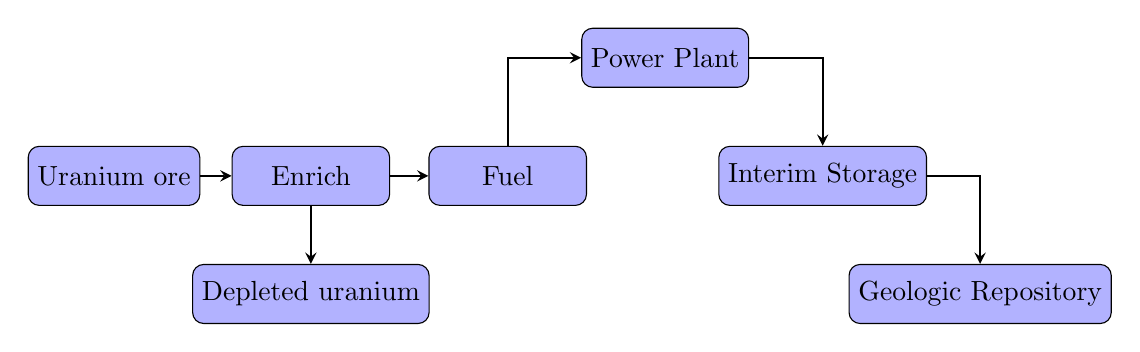
\begin{tikzpicture}[node distance=1.5cm]
        \node (ore) [facility] {Uranium ore};
        \node (enrichment) [facility, right of=ore, xshift=1cm]{Enrich};
        \node (llwsink) [facility, below of=enrichment]{Depleted uranium};
        \node (fabrication) [facility, right of=enrichment, xshift=1cm]{Fuel};
        \node (reactor) [facility, above of=fabrication, xshift=2cm]{Power Plant};
        \node (spentfuel) [facility, below of=reactor, xshift=2cm]{Interim Storage};
        \node (sinkhlw) [facility, below of=spentfuel, xshift=2cm]{Geologic Repository};

        \draw [arrow] (ore) --  (enrichment); 
        \draw [arrow] (enrichment) -- (fabrication);
        \draw [arrow] (enrichment) -- (llwsink);
        \draw [arrow] (fabrication) |- (reactor);
        \draw [arrow] (reactor) -| (spentfuel);
        \draw [arrow] (spentfuel) -| (sinkhlw);

        \end{tikzpicture}
    \caption{Material flow for a once-through nuclear fuel cycle. All material is 
    disposed of after use in a reactor. Adapted from \protect\cite{wigeland_identification_2011}.}
    \label{fig:once_through_background}
\end{figure}

\subsection{Recycling fuel cycle}
A recycling fuel cycle is characterized by fuel going through additional 
passes through a reactor after a separtations step to remove fission 
products (Figure \ref{fig:recycle_background})
\begin{figure} 
    \centering
    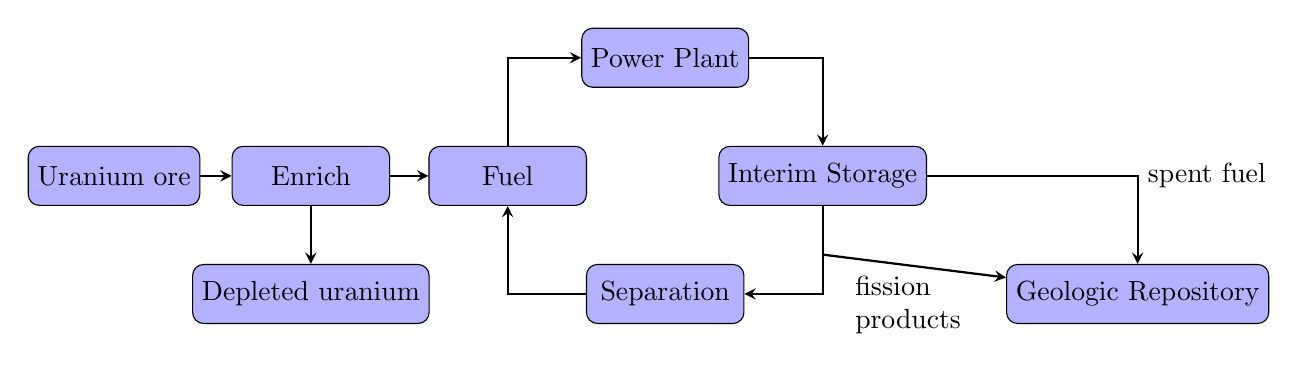
\begin{tikzpicture}[node distance=1.5cm]
        \node (ore) [facility] {Uranium ore};
        \node (enrichment) [facility, right of=ore, xshift=1cm]{Enrich};
        \node (llwsink) [facility, below of=enrichment]{Depleted uranium};
        \node (fabrication) [facility, right of=enrichment, xshift=1cm]{Fuel};
        \node (reactor) [facility, above of=fabrication, xshift=2cm]{Power Plant};
        \node (spentfuel) [facility, below of=reactor, xshift=2cm]{Interim Storage};
        \node (sinkhlw) [facility, below of=spentfuel, xshift=4cm]{Geologic Repository};
        \node (separation) [facility, below of=reactor, yshift=-1.5cm]{Separation};

        \draw [arrow] (ore) --  (enrichment); 
        \draw [arrow] (enrichment) -- (fabrication);
        \draw [arrow] (enrichment) -- (llwsink);
        \draw [arrow] (fabrication) |- (reactor);
        \draw [arrow] (reactor) -| (spentfuel);
        \draw [arrow] (spentfuel) -| node[anchor=west]{spent fuel}(sinkhlw);
        \draw [arrow] (spentfuel) |- (separation);
        \draw [arrow] (separation) -| (fabrication);
        \draw [arrow] (9,-1.0)-- node[anchor=north, text width=1.5cm]{fission products}(sinkhlw);
        
        \end{tikzpicture}
    \caption{Material flow for a once-through nuclear fuel cycle. All material is 
    disposed of after use in a reactor. Adapted from \protect\cite{wigeland_identification_2011}.}
    \label{fig:recycle_background}
\end{figure}

\subsection{Enrichment}
In the nuclear fuel cycle, enrichment increases the relative abundance of 
uranium-235 compared to uranium-238 in the fuel. The capacity of an 
enrichment facility is based on a number of quantities \cite{tsoulfanidis_nuclear_2013}:
\begin{subequations}
    \begin{equation}
        F = \text{mass (kg) of feed material per unit time}
    \end{equation}
    \begin{equation}
        P = \text{mass (kg) of product material per unit time}
    \end{equation}
    \begin{equation}
        T = \text{mass (kg) of tails produced per unit time}
    \end{equation}
    \begin{equation}
        x_f = \text{weight fraction of $^{235}$U in the feed stream}
    \end{equation}
    \begin{equation}
        x_p = \text{weight fraction of $^{235}$U in the product stream}
    \end{equation}
    \begin{equation}
        x_t = \text{weight fraction of $^{235}$U in the tails stream}
    \end{equation}
    \begin{equation}
        SWU = \text{separtive work units (SWU); the physical work required to separate the isotopes}
    \end{equation}
\end{subequations}

Each of these quantites can be related using the following equations:
\begin{subequations}
    \begin{equation}
        F = P + T
    \end{equation}
    \begin{equation}
        x_fF = x_pP + x_tT
    \end{equation}
    \label{eq:enrichment_2}
    \begin{equation}
        SWU = [P*V(x_p) +T*V(x_t) - F*V(x_f)]*t
    \end{equation}
    \text{in which:}
    \begin{equation}
        V(x_i) = (2x_i - 1)*\ln\left(\frac{x_i}{1-x_i}\right)
    \end{equation}
    \begin{equation}
        t = \text{a given time period}
    \end{equation}
\end{subequations}

\section{Fuel cycle simulators}
Fuel cycle simulators are computational tools to model the flow of materials
and the commissioning and decommissioning of facilities for a given fuel 
cycle. 

A variety of fuel cycle simulators have been developed to meet 
different needs, including VISION\cite{yacout_visionverifiable_2006}, 
DYMOND \cite{yacout_visionverifiable_2006}, and ORION \hl{FIND CITATION}. 
This work primarily 

\subsection{\Cyclus}
\Cyclus is a dynamic, open source agent-based fuel cycle simulator. Built 
in C++, \Cyclus uses only open source and freely available libraries to 
provide full access to all users and developers. The 
\Cyclus architecture treats materials and facilities discretely and allows 
for variable fidelity levels \cite{huff_fundamental_2016}. These attributes
of \Cyclus allow for the software to easily model any fuel cycle scenario.

\Cyclus uses the notion of an \textit{agent} to to represent different 
components in the simulated fuel cycle. Agents are 
defined using the \Cyclus application programming interface (API), which 
defines and develops agents. Generic APIs are used to allow users 
to develop their own suite of agent libraries and use them within \Cyclus. 
The APIs anticipate the structure on information about a given library 
that is required by the core \Cyclus kernel. This allows them to facilitate 
information sharing between the plug-in library and the \Cyclus framework. 
In addition to the flexibility in libraries and agents, this framework 
also allows for flexibility in licensing and distribution of the user 
defined libraries. Libraries are loaded without changes to the \Cyclus 
kernel and without unwanted transfer of sensitive information. 

The agent-based modeling paradigm employed by \Cyclus allows agent level 
modeling, as opposed to system level modeling. This allows difference 
fuel cycle facilities, such as a reactor and a fuel fabrication plant, to 
be defined independently but still interact with each other in the 
simulation. There are three main groups of agents within the \Cyclus 
architecture: facilities, institutions, and regions. Facilities are 
the individual units in the fuel cycle that implement technology, 
such as a fuel fabrication facility or a uranium mine. Institutions 
manage the facilities, similar to a company. Regions provide geographic 
and political context for the institutions and regions, and can be thought 
of as similar to individual nations. Each type of agent has its own 
class wihtin \Cyclus. 

The types of agents are related using a parent-child hierarchy: regions are
parents of institutions, and institutions are parents of facilities. This 
structure requires that institutions are responsible for the deployment 
and decommissioning of the facilities. It also allows for advanced logic 
to be implemented wth respect to facility building and decommissioning, 
such as preferential regional or institutional trading (e.g. tariffs or 
contracts). 

\subsection{Verification and Use}
Verification of \Cyclus has been performed \cite{bae_standardized_2019}, 
based on a transition scenario from an open fuel cycle to an advanced
fuel cycle with reprocessing \cite{feng_standardized_2016}. Due to 
some inherent differences in \Cyclus and the other fuel cycle simulators 
used by \cite{feng_standardized_2016} there were some differences in 
the scenario parameters, such as \gls{LWR} batch size or 
cycle length. These differences are implemented to conserve the reactor 
core size, with a negligible difference in the \gls{SFR} core size. \Cyclus 
was shown to have strong agreement with the verification of other 
fuel cycle simulators \cite{bae_standardized_2019} with respect to 
multiple metrics such as reactor startup and decommission schedule, fresh 
fuel loading, and annual reprocessing throughputs. One major difference
between \Cyclus and other fuel cycle simulators identified by this work 
is that \Cyclus fully resolves discrete batches for fuel discharge. This 
implementation allows \Cyclus to better match realistic fuel handeling, but 
does not prevent \Cyclus from producing comparable results to other 
fuel cycle simulators. 

\Cyclus has been used to model the EG 23 transition scenario 
\cite{wigeland_nuclear_2014}, assuming a 1\% growth in power demand 
\cite{djokic_application_2015}. The results from \Cyclus were compared 
to the results from modeling the same transition scenario with DYMOND, 
a fuel cycle simulator from \gls{ANL}. The power generated, reactor entry 
time, and reactor exit time for the \Cyclus simulation qualitatively 
matches well with the results of the DYMOND simulation, but the power 
demand growth could match better to the target 1\% by slightly modifying 
the \gls{SFR} deployment. 

\section{Fuel cycle sensitivity analysis}

\section{Reactors with HALEU}
A lot of work has been done to evaluate the performance of reactors 
using \gls{HALEU} fuel. Burns et al. investigated the reactor and fuel cycle 
performance of an \gls{LWR} fueled by an enrichment above 5\% \cite{burns_reactor_2020}.
Their work showed that increasing the fuel enrichment up to 7\% does not 
largely affect the fuel temperature or the moderator temperature coefficents,
but it does decrease the soluble boron coefficient and increase the maximum 
burnup ar the edges of the fuel pellets. The impacts on the fuel cycle include 
an increase in the amount of natural uranium required, a decrease in the 
amount of high-level waste disposed of per unit energy, and changes in the 
waste radioacitivity waste. The increase in natural uranium matches 
expectations
because the product mass (i.e. mass of fuel in the core) per unit 
energy is the same, and 
based on \ref{eq:enrichment_2} the increase in the product enrichment would 
lead to an increase in the feed mass. 

Increasing the fuel enrichment of the NuScale SMR has also been investigated 
\cite{carlson_implications_2022}.


\chapter{Fuel cycle modeling methodology}
The fuel cycle scenarios created show the resources required for the transition from the 
current fleet of \glspl{LWR} in the US to advanced reactors using \gls{HALEU}.
All fuel cycle models were run in \Cyclus 
\cite{huff_fundamental_2016}. Each simulation models current 
\glspl{LWR} starting in 1965 and models all reactors out to 2090 with a timestep 
of one month. Start 
and select end dates for \glspl{LWR} were obtained from the \gls{IAEA} \gls{PRIS} database 
\cite{noauthor_power_1989}. Reactors still in operation in December 2020, and thus 
lacking an end date in the \gls{PRIS} database are assumed to operate through their 
current operating license 
\cite{noauthor_us_nodate}.
Only reactors with a power level above 400 MWe were used in the simulation 
to avoid including prototype and research reactors present in the database. 
Approximate masses for fuel used in the core the \glspl{LWR} was obtained 
from \cite{todreas_nuclear_2012} and \cite{cacuci_handbook_2010}. 

Material compositions for each commodity in the models are defined using recipes.
Recipes for \gls{LWR} fresh and spent fuel were found in \cite{jacobson_verifiable_2010}.
Obtaining recipes for fresh and spent fuel for the advanced reactors is described in 
Section \ref{sec:reactor_methods}. The tails assay from enrichment is defined as 
0.2\% assay. 

Fuel cycle scenarios are grouped into once-through fuel cycles and recycle fuel 
cycles. Within each group, fuel cycle models are defined based on the energy demand 
of the scenario (either no growth or 1\% annual growth in demand) and by the 
advanced reactors deployed in the scenario. The transition from \glspl{LWR} to 
advanced reactors is modeled as beginning in 2025, so the energy demand is based on the 
energy supplied by \glspl{LWR} in 2025. Many of the current planned \gls{HALEU}-fueled 
reactors are not scheduled to be deployed until \hl{???}, but 2025 was selected as 
the transition start time for this work because it will provide an upper 
bounding case for if these reactors were to be deployed in mass on 
an aggressive timeline. 

Each of the fuel cycle scenarios 
defined in this work are compared on the number of reactors deployed, the 
uranium usage (both uranium ore and what is sent to the reactors), the enrichment 
\gls{SWU} capacity required, and the amount of waste produced. The natural 
uranium usage and waste production are two of the metrics used in the \gls{ES} 
\cite{wigeland_nuclear_2014} and provide a way to compare this work to that study.

\section{Reactors} \label{sec:reactor_methods}
This work considers three advanced reactors: the \gls{USNC} \gls{MMR}, 
\cite{mitchell_usnc_2020}, the X-energy Xe-100 
\cite{harlan_x-energy_2018,hussain_advances_2018}, and the NuScale VOYGR reactor
\cite{nuscale_chapter_2020,nuscale_chapter_2020-1}. The \gls{USNC} \gls{MMR}
and X-energy Xe-100 reactors require \gls{HALEU}, but the NuScale VOYGR requires
a similar enrichment level to current \gls{LWR} fuel (Table \ref{tab:reactor_summary}). 
The NuScale VOGYR was included in this work, despite not requiring \gls{HALEU} fuel, 
because it is close to obtaining regulatory approval and is very likely to be 
deployed along-side reactors that require \gls{HALEU}. Including the NuScale 
VOYGR reactor in the transition scenarios provides insight into the material 
requirements of deploying \gls{HALEU} and non-\gls{HALEU}-fueled reactors 
in tandum. However, because the NuScale VOYGR reactor does not require 
\gls{HALEU}, the transition from \glspl{LWR} to only the VOYGR reactor is 
not considered in this work.

\begin{table}[ht]
    \centering
    \caption{Advanced reactor design specifications.}
    \label{tab:reactor_summary}
    \begin{tabular}{l p{3.5cm}p{3cm}p{3cm}p{3cm}}
        \hline
        Design Criteria & \gls{USNC} \gls{MMR} & 
            X-energy Xe-100 & NuScale VOYGR \\\hline
        Reactor type & Modular HTGR & Modular HTGR & SMR\\
        Power Output (MWth) & 15 & 200 & 160\\
        Enrichment (\% $^{235}U$) & 13 & 15.5 & 4.09\\
        Cycle Length (years) & 20 & online refuel & 2\\
        Fuel form & UO$_2$ + UCO pebbles & UCO pebbles & UO$_2$ pellets\\
        Discharge fuel burnup (GWd/MTU) & 42.7& 160 & 12 (cycle) \\
        Reactor Lifetime & 20 years & 60 years & 60 years\\
        \hline
    \end{tabular}
\end{table}

Defining a reactor with the ``cycamore:Reactor'' archetype \cite{scopatz_cyclus_2015}, 
requires the refueling scheme and the fuel recipes. The refueling scheme includes 
the cycle length, the refuling length, and the amount of fuel put into the reactor 
at each refueling. 
The \gls{MMR} is not meant to undergo refueling, the initial core is designed 
to operate for the entire lifetime of the reactor \cite{mitchell_usnc_2020}. 
Therefore, this reactor 
is modeled to not include any refueling. The mass of urnaium in the core was
calculate based on the power level, fuel burnup, and lifetime of the 
fuel in the core using values reported in \cite{hawari_development_2018}. 
The total fuel mass was then calculated based on the composition of the fuel. 
Only uranium-containing fuel components were considered in this calculation, 
Any silicon-carbide in the \gls{TRISO} particles was not 
considered, only the uranium dioxide and uranium carbide in the \gls{TRISO}
particle. Doing this calculation assumes that uranium-contaning materials would 
be the limiting factor in the fuel fabrication process and that other materials 
would be available as needed. 

The Xe-100 reactor is designed to 
undergo online refueling operations, with each \gls{TRISO} pebble passing 
through the reactor six times before discharge \cite{hussain_advances_2018}. 
Every six months about 1/7th 
of the pebbles in the core are expected to be discharged. Online refueling 
cannot be explicitly modeled in \Cyclus, so the Xe-100 refueling is modeled 
as a replacement of 1/7th of the enrtire core every 6 months. The mass of 
each \gls{TRISO} was calculated by calculating the volume of a single 
uranium carbide \cite{harlan_x-energy_2018} and multiplying by the density of the 
particle. This mass was then multiplied by the number of particles in each 
pebble, and by the number of pebbles in the core \cite{harlan_x-energy_2018}.
This calculation provided the total mass of uranium carbide in the core. The 
total mass was then divided by 7 to get an average for the fuel mass replaced 
each modeled refueling.  

The VOYGR reactor contains 37 fuel assemblies, with three different enrichment 
levels \cite{nuscale_chapter_2020}. Each refueling replaces 13 fuel assemblies, 
because the middle assembly is replaced at every outage. The mass of fuel in 
each assembly is reported in \cite{nuscale_chapter_2020}. The reported enrichment 
for the VOYGR reactor in Table \ref{tab:reactor_summary}is the average for 
each refueling. The VOYGR reactor is 
modeled as a replacement of 13 fuel assemblies every refueling outage. Each refueling 
outage is modeled as taking one month, because that is the refueling outage time 
modeled for the \glspl{LWR}, and one month is the minimum time step in the 
simulations. 

Fresh fuel recipes for these reactors are based on the required fuel form for 
each reactor using the appropriate uranium isotope ratio for enrichment. Spent fuel 
recipes were obtained from depletion 
calculations in serpent \cite{leppanen_serpent_2014}. All serpent models used 
the JEFF 3.1.2 cross section data library \cite{koning_status_2011}.
The model created for the \gls{MMR} is based on the work reported in 
\cite{hawari_development_2018}, and a cross section of the core is shown in 
\hl{FIGURE}.  \hl{add more when available}

\section{Once-through fuel cycle}
The flow of material through the modeled once-through fuel cycles is shown 
in Figure \ref{fig:once-through_fuel_cycle}. The once-through fuel cycles model 
material from the mine through final disposal in a final respository (the 
``HLW Sink'' in FIgure \ref{fig:once-through_fuel_cycle}. The ``advanced reactor'' node in Figure 
\ref{fig:once-through_fuel_cycle} represents any subset of the advanced reactors included 
in the scenario. The \glspl{LWR} are deployed at their specific start and end dates 
using the ``cycamore::DeployInst'', the advanced reactors are deployed as needed by 
the ``cycamore::ManagerInst'', and the energy demand of the scenario is defined using 
the ``cycamore::GrowthRegion'' \cite{scopatz_cyclus_2015}.

\begin{figure}
    \centering
    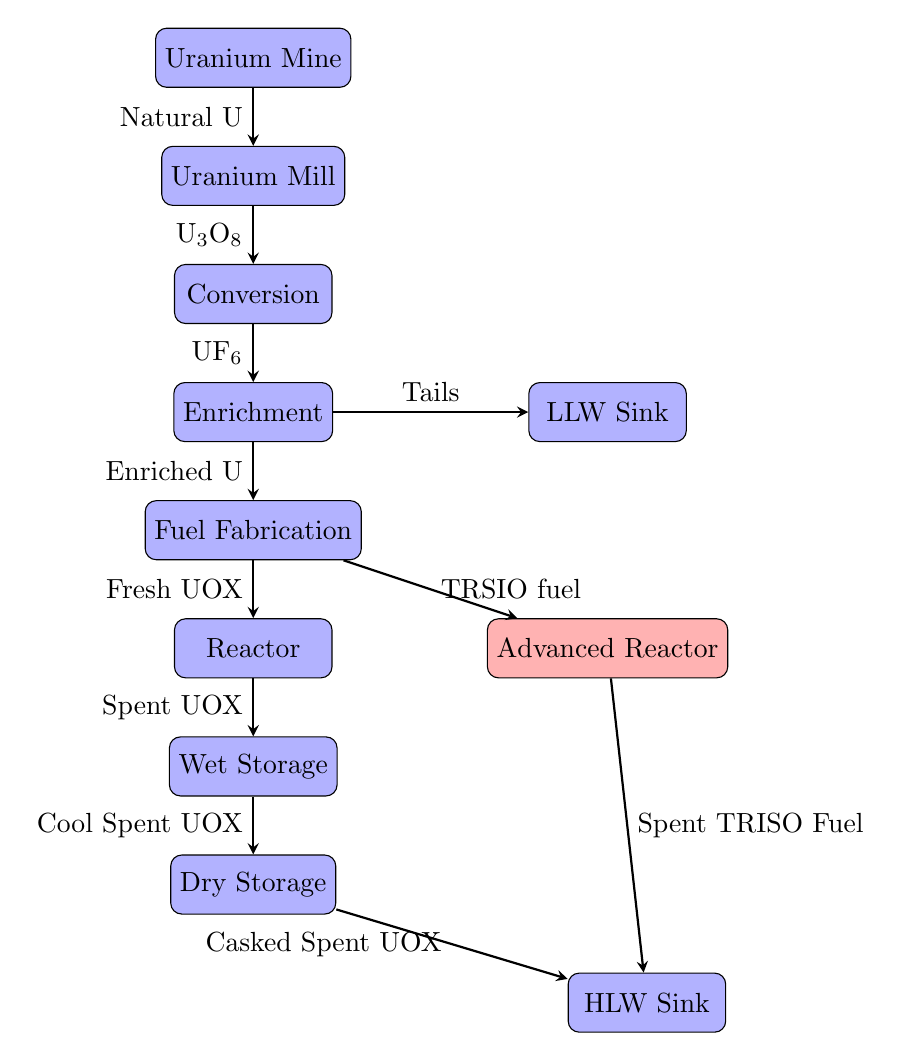
\begin{tikzpicture}[node distance=1.5cm]
        \node (mine) [facility] {Uranium Mine};
        \node (mill) [facility, below of=mine] {Uranium Mill};
        \node (conversion) [facility, below of=mill] {Conversion};
        \node (enrichment) [facility, below of=conversion]{Enrichment};
        \node (fabrication) [facility, below of=enrichment]{Fuel Fabrication};
        \node (reactor) [facility, below of=fabrication]{Reactor};
        \node (adv_reactor) [transition, right of=reactor, xshift=3cm]{Advanced Reactor};
        \node (wetstorage) [facility, below of=reactor]{Wet Storage};
        \node (drystorage) [facility, below of=wetstorage]{Dry Storage};
        \node (sinkhlw) [facility, below of=drystorage, xshift=5cm]{HLW Sink};
        \node (sinkllw) [facility, right of=enrichment, xshift=3cm]{LLW Sink};

        \draw [arrow] (mine) -- node[anchor=east]{Natural U} (mill); 
        \draw [arrow] (mill) -- node[anchor=east]{U$_3$O$_8$}(conversion); 
        \draw [arrow] (conversion) -- node[anchor=east]{UF$_6$}(enrichment);
        \draw [arrow] (enrichment) -- node[anchor=east]{Enriched U}(fabrication);
        \draw [arrow] (enrichment) -- node[anchor=south]{Tails}(sinkllw);
        \draw [arrow] (fabrication) -- node[anchor=east]{Fresh UOX}(reactor);
        \draw [arrow] (fabrication) -- node[anchor=west]{TRSIO fuel}(adv_reactor);
        \draw [arrow] (reactor) -- node[anchor=east]{Spent UOX}(wetstorage);
        \draw [arrow] (wetstorage) -- node[anchor=east]{Cool Spent UOX}(drystorage);
        \draw [arrow] (drystorage) -- node[anchor=east]{Casked Spent UOX}(sinkhlw);
        \draw [arrow] (adv_reactor) -- node[anchor=west]{Spent TRISO Fuel}(sinkhlw);

        \end{tikzpicture}
    \caption{Fuel cycle facilities and material flow between facilities. Facilities in 
    red are added in for the transition scenarios.}
    \label{fig:fuel_cycle}
\end{figure}

The once-through scenarios model the current fleet of \glspl{LWR} in the 
US and the transition to multiple 
combinations of these reactors and different energy demand scenarios, 
summarized in Table \ref{tab:scenarios_once-through}. Scenario 1 models
the \gls{LWR} fleet without the transition to any advanced reactor to provide 
a comparison to if no new reactors are built.  

\begin{table}[ht]
    \centering
    \caption{Summary of the once-through fuel cycle transition scenarios.}
    \label{tab:scenarios_once-through}
    \begin{tabular}{l l l}
            \hline
            Scenario Number & Reactors Present & Energy growth model\\\hline
            1 & \glspl{LWR} & N/A \\
            2 & \glspl{LWR} and \gls{USNC} \gls{MMR} & No growth \\
            3 & \glspl{LWR} and X-energy Xe-100& No growth \\
            4 & \glspl{LWR}, X-energy Xe-100, \gls{USNC} \gls{MMR}& No growth\\
            5 & \glspl{LWR}, \gls{USNC} \gls{MMR}, NuScale VOYGR & No growth\\
            6 & \glspl{LWR}, X-energy Xe-100, NuScale VOYGR & No growth\\
            7 & \glspl{LWR}, X-energy Xe-100, \gls{USNC} \gls{MMR}, NuScale VOYGR & No growth\\
            8 & \glspl{LWR} and \gls{USNC} \gls{MMR}& 1\% growth \\
            9 & \glspl{LWR} and X-energy Xe-100& 1\% growth\\
            10 & \glspl{LWR}, X-energy Xe-100, \gls{USNC} \gls{MMR}& 1\% growth\\
            11 & \glspl{LWR}, \gls{USNC} \gls{MMR}, NuScale VOYGR & 1\% growth\\
            12 & \glspl{LWR}, X-energy Xe-100, NuScale VOYGR & 1\% growth\\
            13 & \glspl{LWR}, X-energy Xe-100, \gls{USNC} \gls{MMR}, NuScale VOYGR & 1\% growth\\
            \hline
    \end{tabular}
\end{table}

\section{Recycle fuel cycle}
The flow of material through the fuel cycle scenarios with recycling is shown in 
Figure \ref{fig:recycle_fuel_cycle}. Only spent fuel from the advanced reactors 
is reprocessed and reused in a reactor. \hl{Do I want fuel to be disposed of 
after one additional pass? Probably need to read literature}

\begin{figure}
    \centering
    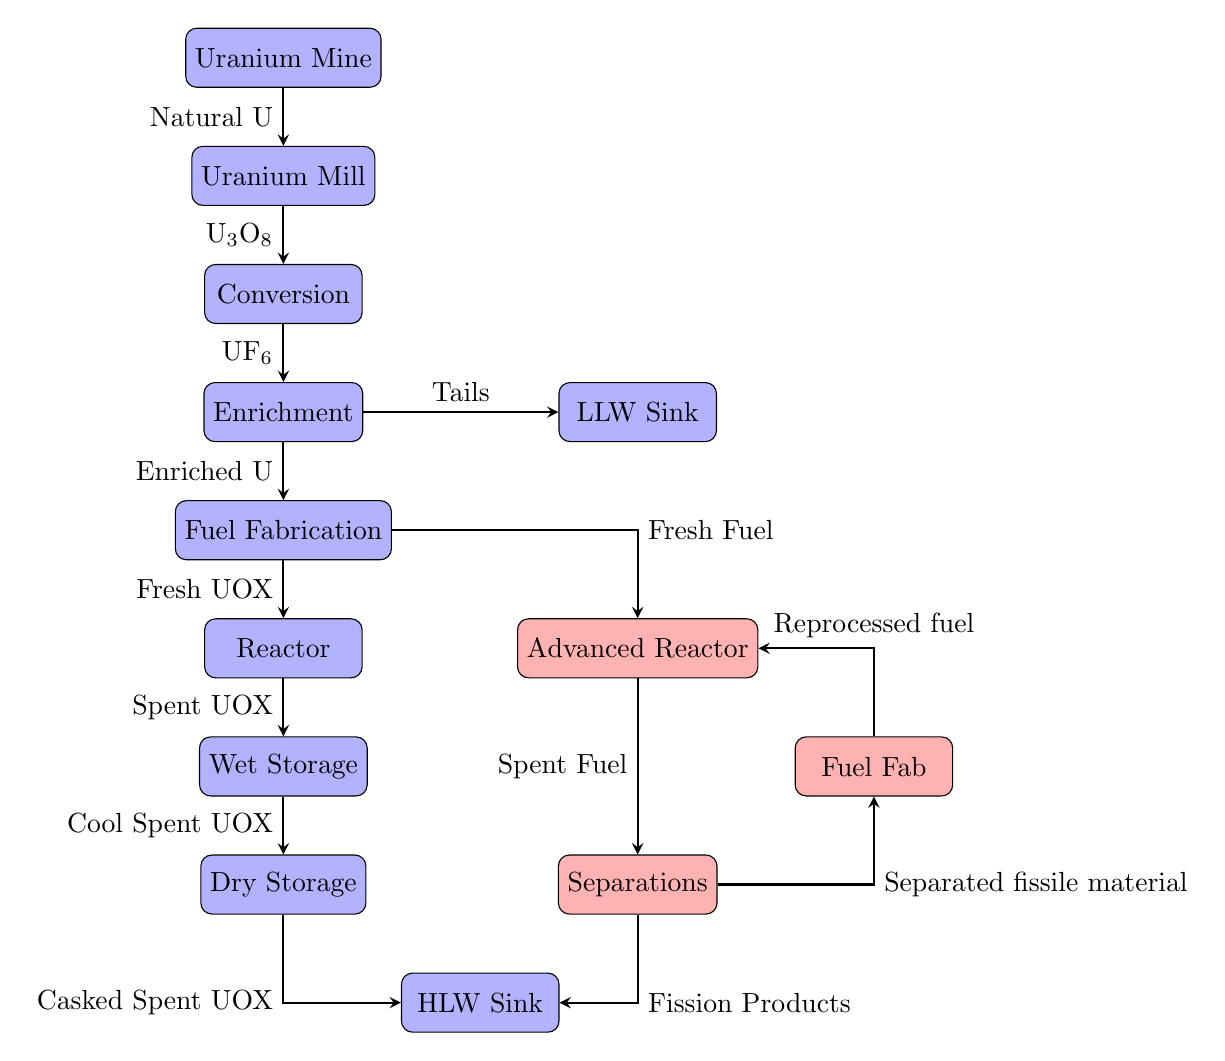
\begin{tikzpicture}[node distance=1.5cm]
        \node (mine) [facility] {Uranium Mine};
        \node (mill) [facility, below of=mine] {Uranium Mill};
        \node (conversion) [facility, below of=mill] {Conversion};
        \node (enrichment) [facility, below of=conversion]{Enrichment};
        \node (fabrication) [facility, below of=enrichment]{Fuel Fabrication};
        \node (reactor) [facility, below of=fabrication]{Reactor};
        \node (adv_reactor) [transition, right of=reactor, xshift=3cm]{Advanced Reactor};
        \node (wetstorage) [facility, below of=reactor]{Wet Storage};
        \node (drystorage) [facility, below of=wetstorage]{Dry Storage};
        \node (sinkhlw) [facility, below of=drystorage, xshift=2.5cm]{HLW Sink};
        \node (sinkllw) [facility, right of=enrichment, xshift=3cm]{LLW Sink};
        \node (separation) [transition, below of=adv_reactor, yshift=-1.5cm]{Separations};
        \node (fuelfab) [transition, below of=adv_reactor,xshift=3cm]{Fuel Fab};

        \draw [arrow] (mine) -- node[anchor=east]{Natural U} (mill); 
        \draw [arrow] (mill) -- node[anchor=east]{U$_3$O$_8$}(conversion); 
        \draw [arrow] (conversion) -- node[anchor=east]{UF$_6$}(enrichment);
        \draw [arrow] (enrichment) -- node[anchor=east]{Enriched U}(fabrication);
        \draw [arrow] (enrichment) -- node[anchor=south]{Tails}(sinkllw);
        \draw [arrow] (fabrication) -- node[anchor=east]{Fresh UOX}(reactor);
        \draw [arrow] (fabrication) -| node[anchor=west]{Fresh Fuel}(adv_reactor);
        \draw [arrow] (reactor) -- node[anchor=east]{Spent UOX}(wetstorage);
        \draw [arrow] (wetstorage) -- node[anchor=east]{Cool Spent UOX}(drystorage);
        \draw [arrow] (drystorage) |- node[anchor=east]{Casked Spent UOX}(sinkhlw);
        \draw [arrow] (adv_reactor) -- node[anchor=east]{Spent Fuel}(separation);
        \draw [arrow] (separation) -| node[anchor=west]{Separated fissile material}(fuelfab);
        \draw [arrow] (fuelfab) |- node[anchor=south]{Reprocessed fuel}(adv_reactor);
        \draw [arrow] (separation) |- node[anchor=west]{Fission Products}(sinkhlw);

        \end{tikzpicture}
    \caption{Fuel cycle facilities and material flow between facilities. Facilities in 
    red are added in for the transition scenarios.}
    \label{fig:recycle_fuel_cycle}
\end{figure}

\begin{table}[ht]
    \centering
    \caption{Summary of the recycle fuel cycle transition scenarios.}
    \label{tab:scenarios_recycle}
    \begin{tabular}{l l l}
            \hline
            Scenario Number & Reactors Present & Energy growth model\\\hline

            \hline
    \end{tabular}
\end{table}

\section{Calculation of results}
The results presented for the transition scenarios are from the SQLite database 
that is output by each \Cyclus simulation. Because the non-reactor facilities 
in the simulations (e.g. enrichment facility) do not have a specific cap on the 
amount of material they can hold, the material being traded by these facilities 
does not accurately capture the material requirements of the reactors. Therefore, 
the material requirements and waste of each scenario are calculated based on 
the material sent to and discharged from the reactors in each scenario. 

The mass of enriched uranium reported is the mass that is sent to the reactors 
at each time step. The \gls{SWU} required is also calculated based on the 
mass sent to the reactors, and does not reflect the capacity of an actual 
facility. The mass of natural uranium required to produce the enriched uranium 
is calculated based on the mass of product sent to the reactors, Eq. \ref{eq:enrichment},
and 


\chapter{Once-through fuel cycle results}

Each of the once-through transition scenarios are compared on multiple 
criteria: the number of advanced reactors deployed, the energy profile, 
the mass of enriched 
uranium required, the amount of \gls{SWU} capacity required to enrich uranium,
and the mass of waste produced. 

\subsection{Scenario 1}
Scenario 1 models only the \glspl{LWR} deploying the United States with no 
perscribed energy demand. As expected, the energy 
produced by the \glspl{LWR} follows with the number of reactors deployed
(Figure \ref{fig:energy1}). The maximum number of \glspl{LWR} deployed is 
, and reactors are deployed in 2025. 

I can compare some of these results to EIA data on power produced and 
uranium purchases from domestic suppliers \cite{us_eia_monthly_2022}.

\begin{figure}
    \centering
    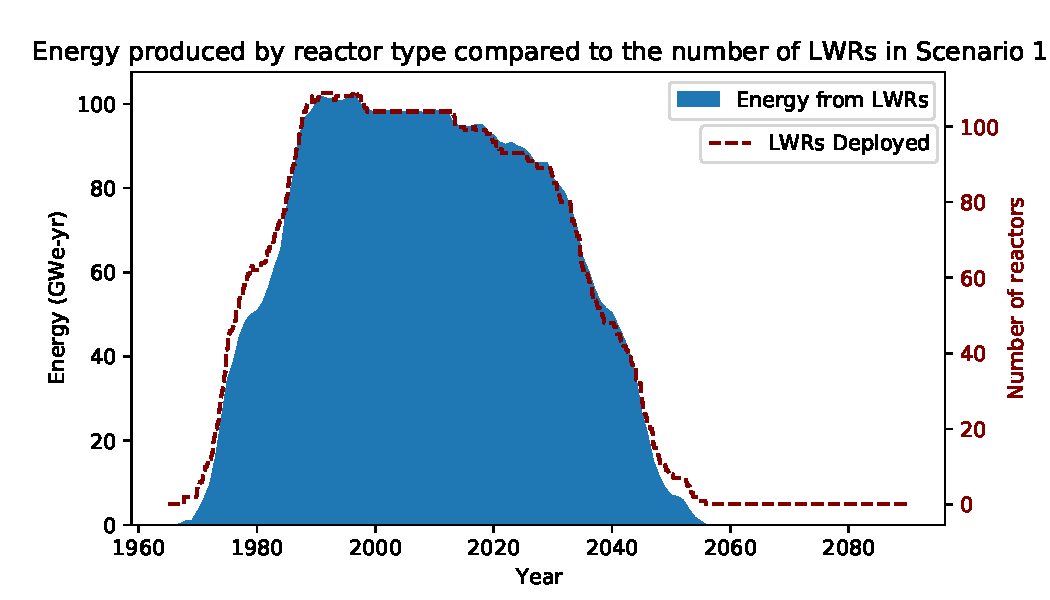
\includegraphics{energy_scenario1.pdf}
    \caption{Energy produced and the number of reactors deployed in Scenario 1.}
    \label{fig:energy1}
\end{figure}

\subsection{Reactor deployment}

\subsection{Uranium resources}

\subsection{SWU capacity}

\subsection{Waste}

\chapter{Recycling fuel cycle results}
\input{recycling-results.tex}

\chapter{Sensitivity Analysis}
\input{sensitivity.tex}

\chapter{Neutronics effects}
\input{neutronics.tex}

\chapter{Conclusions}
\input{conclusions.tex}

%\chapter*{Appendix}
%Appendix.

\backmatter

\bibliographystyle{ieeetr}
\bibliography{../bibliography}

\end{document}
\endinput
%%
%% End of file `thesis-ex.tex'.
